\documentclass{article}
\usepackage[utf8]{inputenc}
\usepackage[greek,english]{babel}
\usepackage{alphabeta}
\usepackage{fancyhdr}
\usepackage{listings}
\usepackage{mathtools}
\usepackage{siunitx}
\usepackage{xcolor}
\usepackage{graphicx}
\usepackage{pgfplots}
\usepackage[export]{adjustbox}
\usepackage{biblatex}
\addbibresource{ct2-citations.bib}

\title{Εργαστηριακή Εργασία 2 - Εξαρτήματα RLC σε DC τάση, μεταβατικά φαινόμενα}
\author{Χρήστος Μαργιώλης - 19390133 \\ Τμήμα 4}
\date{Ιούνιος 2020}

\begin{document}

\begin{figure}[t!]
    \centering
    
\includegraphics[scale=0.3, center]{./res/Logo_University_of_West_Attica.png}
    \Large
    \textbf{Πανεπιστήμιο Δυτικής Αττικής} \\
    \large
    Τμήμα Μηχανικών Πληροφορικής και Ηλεκτρονικών Υπολογιστών \\
    Θεωρία Κυκλωμάτων
\end{figure}
\begin{figure}[b]
    \centering
    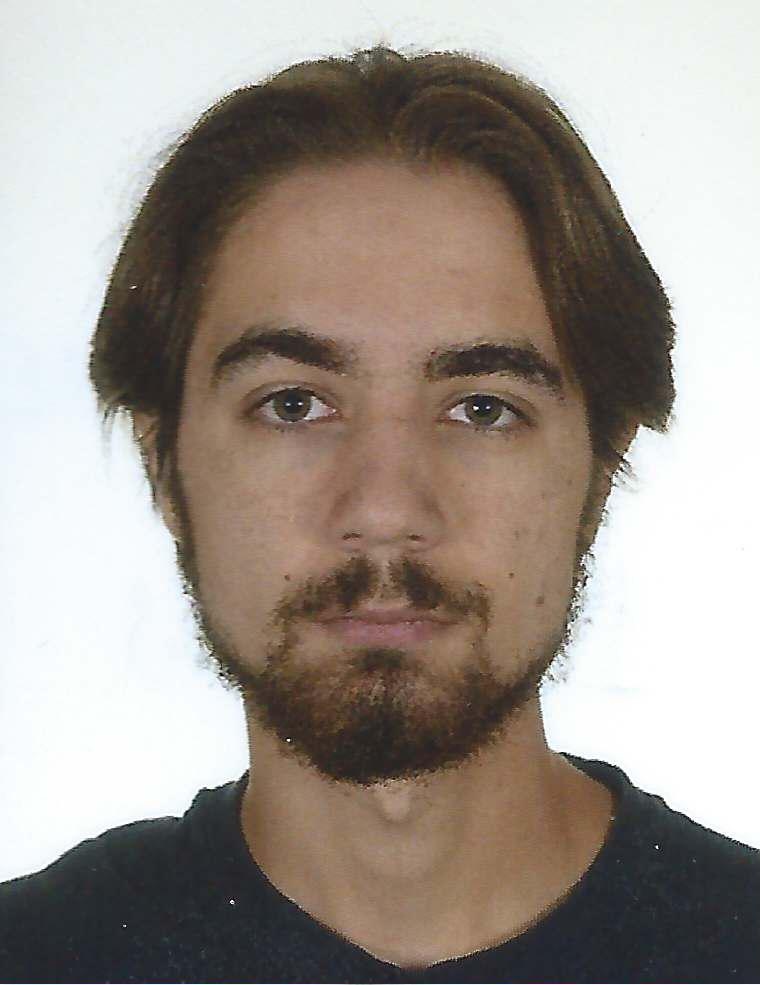
\includegraphics[scale=1]{./res/19390133.jpeg}
\end{figure}

\begin{titlepage}
\maketitle
\end{titlepage}

\renewcommand{\contentsname}{Περιεχόμενα}
\tableofcontents

\renewcommand{\abstractname}{Εισαγωγή}
\begin{abstract}
	Το αντικείμενο της εργασίας αυτής είναι η κατανόηση της βασικής λειτουργίας
	και συμπεριφοράς των RC και RL κυκλωμάτων.
\end{abstract}
\pagebreak

\section{Συλλογή βιβλιογραφίας}
Η βιβλιογραφία που χρησιμοποιήθηκε, αν και μικρή σε έκταση, κάλυψε όλα τα βασικά
προβλήματα της εργασίας. Τα μέρη της βιβλιογραφίας που χρησιμοποιήθηκαν εστιάζουν
κυρίως στους μαθηματικούς τύπους που χρησιμοποιήθηκαν για τις πειραματικές μετρήσεις.

\section{Περιγραφή υλοποίησης}
Για την υλοποίηση της εργασίας και βασισμένος στην παραπάνω βιβλιογραφία που συλλέχθηκε,
χρησιμοποίησα μερικά από τα βασικά υλικά ενός κυκλώματος RC και RL, δηλαδή τον πυκνωτή
και το πηνίο.

\section{Εργαστηριακό μέρος}
\subsection{Υλοποίηση κυκλωμάτων}
Οι τύποι που χρησιμοποιήθηκαν για τις παρακάτω μετρήσεις είναι οι εξής: \\
Για τις συνδεσμολογίες RC
\[V_C(t) = V(1- e^{-\frac{1}{RC}t})\]
Για τις συνδεσμολογίες RL
\[V_L(t) = Ve^{\frac{-R}{L}t}\]

\subsubsection{Μετρήσεις}
\begin{center}
\begin{tabular}{|c|c|c|c|c|c|c|}
\hline
\multicolumn{7}{|c|}{RC} \\
\hline
R (\si{\ohm}) & $τ = RC$ & $V_C(1τ)$ & $V_C(2τ)$ & $V_C(3τ)$ & $V_C(4τ)$ & $V_C(5τ)$ \\
\hline
100           & 0.00001 & 6.321 & 8.647 & 9.502 & 9.817 & 9.933 \\
\hline
\si{10\kilo}  & 0.001   & 6.321 & 8.647 & 9.502 & 9.817 & 9.933 \\
\hline
\si{22\kilo}  & 0.0022  & 6.321 & 8.647 & 9.502 & 9.817 & 9.933 \\
\hline
\si{100\kilo} & 0.01    & 6.321 & 8.647 & 9.502 & 9.817 & 9.933 \\
\hline
\multicolumn{7}{|c|}{RL} \\
\hline
R (\si{\ohm}) & $τ = L/R$ & $V_L(1τ)$ & $V_L(2τ)$ & $V_L(3τ)$ & $V_L(4τ)$ & $V_L(5τ)$ \\
\hline
100           & 0.0001      & 3.679 & 1.353 & 0.498 & 0.183 & 0.067 \\
\hline
\si{10\kilo}  & 0.000001    & 3.679 & 1.353 & 0.498 & 0.183 & 0.067 \\
\hline
\si{22\kilo}  & 0.000000455 & 3.679 & 1.353 & 0.498 & 0.183 & 0.067 \\
\hline
\si{100\kilo} & 0.0000001   & 3.679 & 1.353 & 0.498 & 0.183 & 0.067 \\
\hline
\end{tabular}
\end{center}

\begin{tikzpicture}
\begin{axis}[
	xlabel={Χρόνος τ($RC$)},
	ylabel={Τάση \si{\volt(t)}},
	xmin=0,
	ymin=6,
	grid style=dashed
]
\addplot[
	color=blue,
]
coordinates{
	(0.00001,6.321)(0.00002,8.647)(0.00003,9.502)(0.00004,9.817)(0.00005,9.933)
};
\end{axis}
\end{tikzpicture}

\begin{tikzpicture}
\begin{axis}[
	xlabel={Χρόνος τ($L/R$)},
	ylabel={Τάση \si{\volt(t)}},
	xmin=0,
	ymin=0,
	grid style=dashed
]
\addplot[
	color=blue,
]
coordinates{
	(0.0001,3.679)(0.0002,1.353)(0.0003,0.498)(0.0004,0.183)(0.0005,0.067)
};
\end{axis}
\end{tikzpicture}

\subsection{Ερωτήσεις}
\begin{itemize}
	\item \textit{Όταν ένας μηχανικός χρειάζεται κύκλωμα για να παρέχει χρονοκαθυστέρηση,
			σχεδόν πάντα επιλέγει κύκλωμα RC αντί για κύκλωμα RL. Εξηγήστε γιατί.} \\

	Ο λόγος που ένας μηχανικός χρειάζεται κύκλωμα RC προκειμένου να παρέχει χρονοκαθυστέρηση,
	είναι ότι ο πυκνωτής μπορεί να αποθηκεύσει ενέργεια και χάρη στην αντίσταση μπορούμε να ελέγξουμε
	την συχνότητα φόρτισης-αποφόρτισης \cite{papadopoulos}. \\

	\item \textit{Περιγράψτε την μέγιστη τιμή του ρεύματος, καθώς επίσης τί θα παρατηρηθεί
			στο ρεύμα με το κλείσιμο του διακόπτη στο παρακάτω κύκλωμα.} \\
	
	\[I(t) = \frac{V}{R}(1 - e^{\frac{-R}{L}t})\]
	άρα για $t = 0$
	\[I(0) = \frac{V}{R}(1 - e^{\frac{-R}{L}0}) \Rightarrow I(0) = \frac{V}{R}0
		\Rightarrow I(0) = \si{0\ampere}\]

	Άρα η μέγιστη τιμή του ρεύματος με το κλείσιμο του διακόπτη είναι \si{0\ampere}.
	
	\item \textit{Τί τιμή αντίστασης απαιτείται σε ένα RC κύκλωμα με τιμή πυκνωτή \si{50\mu\farad},
			προκειμένου να υπάρχει χρονοκαθυστέρηση ενός δευτερολέπτου;} \\

        Προκειμένου να βρούμε την τιμή της αντίστασης, θα χρειαστούμε τον τύπο
        \[τ = RC\]
        και αντικαθιστώντας με $τ = 1s$ και $C = \si{50\mu\farad}$ έχουμε ότι
        \[τ = RC \Rightarrow R = \frac{τ}{C} \Rightarrow R =
            \frac{1}{50 \cdot 10^{-6}} = \si{20\kohm}\]

        Οπότε η απαιτούμενη τιμή αντίστασης προκειμένου να υπάρχει χρονοκαθυστέρηση
        ενός δευτερολέπτου σε RC κύκλωμα με τιμή πυκνωτή \si{50\mu\farad} είναι
        \si{20\kohm}.
\end{itemize}

\renewcommand\refname{Πηγές}
\printbibliography
\end{document}
